\documentclass[12pt,a4paper]{article}
\usepackage[margin=1in]{geometry}
\usepackage[T1]{fontenc}
\usepackage[utf8]{inputenc}
\usepackage{lmodern}
\usepackage{setspace}
\usepackage{enumitem}
\usepackage{booktabs}
\usepackage{longtable}
\usepackage{array}
\usepackage{tabularx}
\usepackage{hyperref}
\usepackage{xcolor}
\usepackage{tikz}
\usetikzlibrary{arrows.meta,positioning,shapes.geometric}

\hypersetup{colorlinks=true,linkcolor=blue,urlcolor=blue,citecolor=blue}
\setstretch{1.12}
\setlength{\parskip}{0.45em}
\setlength{\parindent}{0pt}

\title{Software Requirements Specification (SRS)\\\large EEG Based Motor Imagery Classification}
\author{Team: [Add team members]}
\date{09-Apr-2026}

\begin{document}
\maketitle

\section*{Version}
\textbf{Version:} 1.0 Draft

\section{Introduction}
This SRS defines the functional and technical requirements for a Brain Computer Interface (BCI) project that classifies motor imagery (MI) from EEG signals. The project includes a web frontend and Python backend. Screen A simulates or streams EEG signals and allows target class selection. Screen B displays real-time model predictions and confidence trends.

\section{Literature Review Plan (Mandatory)}
\subsection{Paper Collection Rule}
\begin{itemize}[leftmargin=1.5em]
  \item Each member must collect 3 papers from 2023/2024/2025 from IEEE, Springer, Elsevier, ACM, or similar sources.
  \item Expected total papers by team size:
  \begin{itemize}[leftmargin=1.5em]
    \item Single member: 5 papers
    \item Two members: 6 papers
    \item Three members: 9 papers
    \item Four members: 12 papers
  \end{itemize}
\end{itemize}

\subsection{Paper Objective Mapping Table (Mandatory)}
\begin{longtable}{p{0.10\textwidth}p{0.22\textwidth}p{0.08\textwidth}p{0.18\textwidth}p{0.32\textwidth}}
\toprule
\textbf{Paper No.} & \textbf{Title} & \textbf{Year} & \textbf{Source} & \textbf{Objectives Addressed} \\
\midrule
P1 & [Fill] & [Fill] & [Fill] & [Fill] \\
P2 & [Fill] & [Fill] & [Fill] & [Fill] \\
P3 & [Fill] & [Fill] & [Fill] & [Fill] \\
P4 & [Fill] & [Fill] & [Fill] & [Fill] \\
P5 & [Fill] & [Fill] & [Fill] & [Fill] \\
P6 & [Fill] & [Fill] & [Fill] & [Fill] \\
P7 & [Fill] & [Fill] & [Fill] & [Fill] \\
P8 & [Fill] & [Fill] & [Fill] & [Fill] \\
P9 & [Fill] & [Fill] & [Fill] & [Fill] \\
\bottomrule
\end{longtable}

\subsection{Dataset Table from Reviewed Papers (Mandatory)}
\begin{longtable}{p{0.10\textwidth}p{0.23\textwidth}p{0.30\textwidth}p{0.27\textwidth}}
\toprule
\textbf{Paper No.} & \textbf{Dataset Name} & \textbf{Dataset Link} & \textbf{Purpose} \\
\midrule
P1 & [Fill] & [Fill] & [Fill] \\
P2 & [Fill] & [Fill] & [Fill] \\
P3 & [Fill] & [Fill] & [Fill] \\
P4 & [Fill] & [Fill] & [Fill] \\
P5 & [Fill] & [Fill] & [Fill] \\
P6 & [Fill] & [Fill] & [Fill] \\
P7 & [Fill] & [Fill] & [Fill] \\
P8 & [Fill] & [Fill] & [Fill] \\
P9 & [Fill] & [Fill] & [Fill] \\
\bottomrule
\end{longtable}

\section{Details of Our Project}
\subsection{Objective of Our Project}
To design and implement a real-time EEG motor imagery classification system that:
\begin{itemize}[leftmargin=1.5em]
  \item Accepts EEG streams in Screen A (simulation now, real stream later).
  \item Predicts motor imagery class in Screen B with confidence over time.
  \item Supports four cue classes:
  \begin{itemize}[leftmargin=1.5em]
    \item Class 1: Cue onset left
    \item Class 2: Cue onset right
    \item Class 3: Cue onset foot
    \item Class 4: Cue onset tongue
  \end{itemize}
\end{itemize}

\subsection{Experimental Dataset Considered}
Primary dataset for four-class training:
\begin{itemize}[leftmargin=1.5em]
  \item Files used: A01T.gdf to A09T.gdf (training only)
  \item Files reserved for evaluation: A01E.gdf to A09E.gdf
\end{itemize}

Additional dataset present in workspace (two-class left/right only):
\begin{itemize}[leftmargin=1.5em]
  \item B0101T.gdf to B0903T.gdf (training sessions)
  \item B0104E.gdf to B0905E.gdf (evaluation sessions)
\end{itemize}

Dataset references:
\begin{itemize}[leftmargin=1.5em]
  \item BCI Competition IV portal: \url{https://www.bbci.de/competition/iv/}
  \item BNCI Horizon dataset index: \url{http://bnci-horizon-2020.eu/database/data-sets}
\end{itemize}

\subsection{Preprocessing Methods Considered}
\begin{itemize}[leftmargin=1.5em]
  \item Channel selection and mapping
  \item Bandpass filtering (0.5 Hz to 40 Hz)
  \item Notch filtering at 50 Hz
  \item Per-channel normalization
  \item Epoch extraction after cue onset (causal windowing for online setup)
  \item Feature extraction:
  \begin{itemize}[leftmargin=1.5em]
    \item Mu-band and beta-band power summaries
    \item Variability and normalized feature vectors
  \end{itemize}
\end{itemize}

\subsection{ML/DL Approach Considered}
Planned and current approach:
\begin{itemize}[leftmargin=1.5em]
  \item Baseline model:
  \begin{itemize}[leftmargin=1.5em]
    \item Lightweight neural network classifier (MLP-based checkpoint format)
  \end{itemize}
  \item Next model upgrades:
  \begin{itemize}[leftmargin=1.5em]
    \item EEGNet
    \item CNN-LSTM for temporal dynamics
    \item Transformer-lite variant for sequence modeling
  \end{itemize}
  \item Evaluation metrics:
  \begin{itemize}[leftmargin=1.5em]
    \item Accuracy
    \item Confusion matrix
    \item Class-wise precision/recall/F1
    \item Kappa score (for competition-style comparison)
  \end{itemize}
\end{itemize}

\subsection{Block Diagram of Proposed Approach}
Use draw.io or similar tool for final figure. A LaTeX-renderable version is included below.

\begin{figure}[h!]
\centering
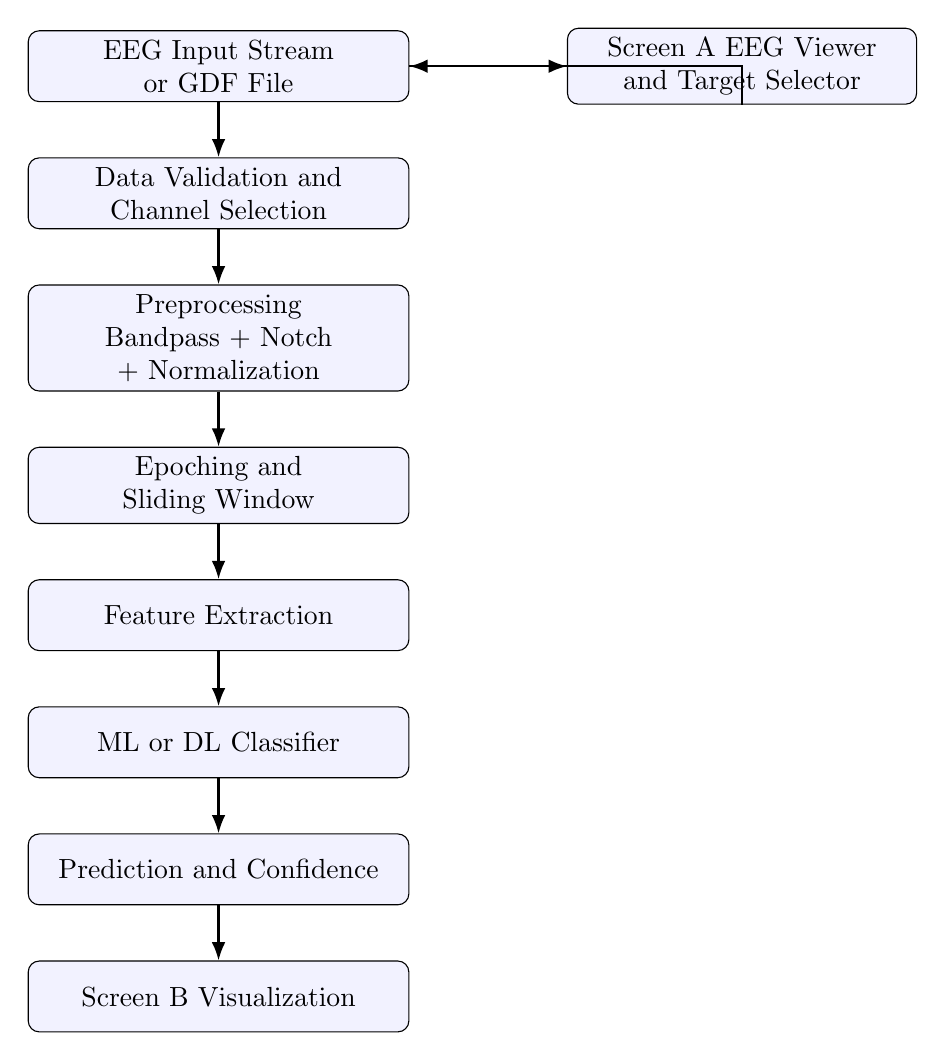
\begin{tikzpicture}[
  node distance=0.7cm,
  block/.style={rectangle, rounded corners, draw=black, align=center, minimum height=0.9cm, text width=4.6cm, fill=blue!5},
  arrow/.style={-Latex, thick}
]
\node[block] (a) {EEG Input Stream or GDF File};
\node[block, below=of a] (b) {Data Validation and Channel Selection};
\node[block, below=of b] (c) {Preprocessing\\Bandpass + Notch + Normalization};
\node[block, below=of c] (d) {Epoching and Sliding Window};
\node[block, below=of d] (e) {Feature Extraction};
\node[block, below=of e] (f) {ML or DL Classifier};
\node[block, below=of f] (g) {Prediction and Confidence};
\node[block, below=of g] (h) {Screen B Visualization};
\node[block, right=2.0cm of a, text width=4.2cm] (i) {Screen A EEG Viewer\\and Target Selector};

\draw[arrow] (a) -- (b);
\draw[arrow] (b) -- (c);
\draw[arrow] (c) -- (d);
\draw[arrow] (d) -- (e);
\draw[arrow] (e) -- (f);
\draw[arrow] (f) -- (g);
\draw[arrow] (g) -- (h);
\draw[arrow] (a.east) -- (i.west);
\draw[arrow] (i.south) |- (a.east);
\end{tikzpicture}
\caption{Proposed approach block diagram}
\end{figure}

\subsection{Tools and Libraries for Implementation}
Development tools:
\begin{itemize}[leftmargin=1.5em]
  \item Python
  \item VS Code
  \item Git and GitHub
  \item draw.io
\end{itemize}

Backend libraries:
\begin{itemize}[leftmargin=1.5em]
  \item FastAPI
  \item Uvicorn
  \item NumPy
  \item SciPy
  \item MNE
  \item scikit-learn
\end{itemize}

Frontend tools:
\begin{itemize}[leftmargin=1.5em]
  \item HTML
  \item CSS
  \item JavaScript
  \item Canvas API for real-time plotting
\end{itemize}

\subsection{Project Timeline (Date-to-Date)}
\begin{longtable}{p{0.44\textwidth}p{0.16\textwidth}p{0.16\textwidth}p{0.14\textwidth}}
\toprule
\textbf{Task} & \textbf{Start Date} & \textbf{End Date} & \textbf{Duration} \\
\midrule
SRS report and PPT preparation & 10-Apr-2026 & 12-Apr-2026 & 3 days \\
Data preprocessing implementation & 13-Apr-2026 & 15-Apr-2026 & 3 days \\
ML/DL baseline implementation & 16-Apr-2026 & 18-Apr-2026 & 3 days \\
Final model tuning and hyperparameter search & 19-Apr-2026 & 22-Apr-2026 & 4 days \\
Result analysis and comparison with literature & 23-Apr-2026 & 25-Apr-2026 & 3 days \\
\bottomrule
\end{longtable}

\section{Functional Requirements}
\begin{itemize}[leftmargin=1.5em]
  \item FR1: System shall stream or simulate EEG in real time.
  \item FR2: System shall allow target MI class selection from frontend.
  \item FR3: System shall preprocess EEG before inference.
  \item FR4: System shall produce class prediction and confidence score.
  \item FR5: System shall display prediction trend on Screen B.
  \item FR6: System shall support retraining from dataset T files.
\end{itemize}

\section{Non-Functional Requirements}
\begin{itemize}[leftmargin=1.5em]
  \item NFR1: Local inference response target below 200 ms per update.
  \item NFR2: Interface must support at least 10 minutes continuous run without crash.
  \item NFR3: Project artifacts must be documented for reproducibility.
\end{itemize}

\section{Risks and Mitigation}
\begin{longtable}{p{0.27\textwidth}p{0.20\textwidth}p{0.43\textwidth}}
\toprule
\textbf{Risk} & \textbf{Impact} & \textbf{Mitigation} \\
\midrule
Domain mismatch between synthetic and real EEG & Wrong live class mapping & Retrain on real dataset and calibrate with validation \\
Class imbalance or partial class coverage & Biased predictions & Enforce class-aware file filtering and class checks \\
Noise and artifacts & Accuracy drop & Use filtering, normalization, artifact-aware trial handling \\
\bottomrule
\end{longtable}

\section{Submission Checklist}
\begin{itemize}[leftmargin=1.5em]
  \item SRS report file
  \item PPT content file
  \item Project report file
  \item Valid dataset links
  \item Mandatory tables completed
  \item Final block diagram in draw.io exported to image/PDF
\end{itemize}

\end{document}
